
%(BEGIN_QUESTION)
% Copyright 2012, Tony R. Kuphaldt, released under the Creative Commons Attribution License (v 1.0)
% This means you may do almost anything with this work of mine, so long as you give me proper credit

An instrument technician is attempting to calibrate a control valve as part of a split-range system, where the valve must be fully closed at 4 mA signal and fully open at 9 mA signal:

$$\includegraphics[width=15.5cm]{i01352x01.eps}$$

Unfortunately, the positioner on this valve cannot achieve this narrow range: even with the valve travel adjustment (span) adjusted all the way to maximum, the valve requires a signal of 10.3 mA to achieve full-open rather than the 9 mA desired.  It is, however, able to achieve full-closed at 4 mA.

\vskip 10pt

Asking for help, the technician seeks answers from his co-workers.  Suggestions range from loosening the spring adjuster nut on the valve actuator stem, to increasing the positioner's air supply pressure, to making adjustments to the positioner's ``zero'' screw, to installing a volume booster between the positioner and actuator diaphragm.

Devise your own solution to this valve range problem, being as specific as you can in your answer.  Furthermore, explain why any one of the co-worker's suggestions will not work to solve this problem.

\underbar{file i01352}
%(END_QUESTION)





%(BEGIN_ANSWER)

I recommend assigning 5 points for a correct answer, and 5 points for a correct debunking of one of the recommended solutions.

\vskip 10pt

Perhaps the simplest solution here is to adjust the span of the I/P.  If the valve positioner achieves full-open at a signal of 10.3 mA (7.725 PSI from the I/P), then the I/P's span should be adjusted so that it outputs that pressure at 9 mA instead of 10.3 mA.  In other words, the I/P calibration should be: {\bf 4 mA = 3 PSI} and {\bf 9 mA = 10.3 PSI}.  This equates to an I/P output of 26.36 PSI at 20 mA.

\vskip 10pt

Loosening the spring adjuster nut will not affect the positioner's calibration, and worse yet it will reduce the seat load that is necessary to achieve tight shut-off.  Increasing the positioner's supply air pressure would allow the positioner to achieve full-open on a valve with a greater upper bench-set value, but since we're already able to achieve full-open as it is this is not a problem and therefore a greater supply pressure will not be a solution.  Adjustments to the zero screw would allow the valve to be full-open at 9 mA, but then it would require less than 4 mA to shut (i.e. it wouldn't fix the span problem).  Lastly, a volume booster would merely allow the valve to be positioned faster, but would not affect the positioner's range.

%(END_ANSWER)





%(BEGIN_NOTES)

{\bf This question is intended for exams only and not worksheets!}.

%(END_NOTES)


